\section{Memento}

O Memento permite armazenar e restaurar o estado interno de um 
objeto sem expor esse estado. Dessa forma, o encapsulamento do 
objeto em questão não é violado, mesmo seu estado sendo armazenado 
externamente.

Isso é alcançado através de uma classe Memento que armazena os 
atributos da classe que precisa ser salva (Originator). A geração 
de um objeto Memento só é possível através do próprio Originator, 
assim como a recuperação de seus atributos. Uma classe Caretaker 
é usada para armazenar objetos do tipo Memento e repassá-los para 
um Originator que precisa acessar o estado do Memento.

\begin{figure}[htb]
	\caption{\label{memento_struct}Estrutura do Memento}
	\begin{center}
	    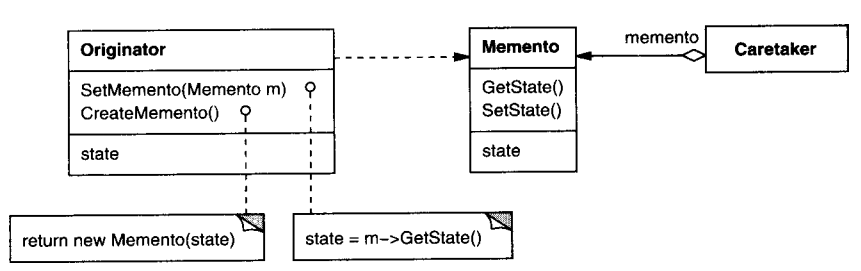
\includegraphics[scale=0.5]{5_padroes-contexto-funcional/5.3_comportamentais/5.3.06_memento/diagram.png}
	\end{center}
\end{figure}

\subsection*{Exemplo Orientado a Objetos}

\begin{lstlisting}[caption={Memento Orientação a Objetos},label=oomemento]



\end{lstlisting}

\subsection*{Contexto Funcional}

\begin{comment}
A ideia de armazenar estados anteriores pode ser alcançada com uma 
estrutura que armazena o valor atual do Originator e uma cópia do 
elemento desejado (ou uma lista armazenando um histórico de cópias). 
A partir dessa estrutura, é simples implementar funções que criam 
a cópia, atualizam o valor do Originator externamente e atualizam 
o valor do Originator a partir dos Mementos.
\end{comment}

\begin{lstlisting}[caption={Memento Funcional},label=fpmemento]



\end{lstlisting}